\documentclass{beamer}
\usepackage{graphicx}
\usepackage{hyperref}
\usepackage{pgfpages} % Enable presenter notes

\setbeameroption{show notes on second screen=right}

\title{FIONA Chatbot Application}
\author{Said Benaissa}
\date{\today}

\begin{document}

\frame{\titlepage}

\begin{frame}{Preventing Hallucinations and Providing Evidence}
    The system uses Retrieval-Augmented Generation (RAG), where search_embeddings in retrieval.py retrieves 
    relevant document chunks using cosine similarity, and generate_answer in llm_generator.py generates grounded responses with the flan-t5-large language model
    \note{
        The backend uses `SentenceTransformer` to create embeddings and `cosine similarity` for chunk retrieval. This ensures that responses are grounded in the source documents.
    }
\end{frame}

\begin{frame}{CI/CD Pipeline for Document Changes}
    \begin{itemize}
        \item Automatically rebuilds embeddings when documents are updated using `embedding_manager.py`.
        \item Other changes trigger a full rebuild of the Docker image.
        \item Ensures that the chatbot is always up-to-date with the latest information.
    \end{itemize}
    \note{
        The CI/CD pipeline is configured to detect changes in the `documents` folder and trigger the embedding rebuild process. This ensures that the chatbot always has the latest information.
    }
\end{frame}

\begin{frame}{Deployment on Linux/Debian-based Systems}
    \begin{itemize}
        \item Docker Compose orchestrates backend and frontend services.
        \item Backend runs on `http://localhost:8000` and frontend on `http://localhost:3000`.
        \item Scalable deployment for small to large-scale systems.
        \item Fully on-premise deployment ensures data privacy.
    \end{itemize}
    \note{
        Deployment is containerized using Docker. The `docker-compose.yml` file simplifies orchestration, making it easy to scale and deploy on various hardware configurations.
    }
\end{frame}

\begin{frame}{Real-time User Interface}
    \begin{itemize}
        \item Users can interact with the chatbot in real-time.
    \end{itemize}
    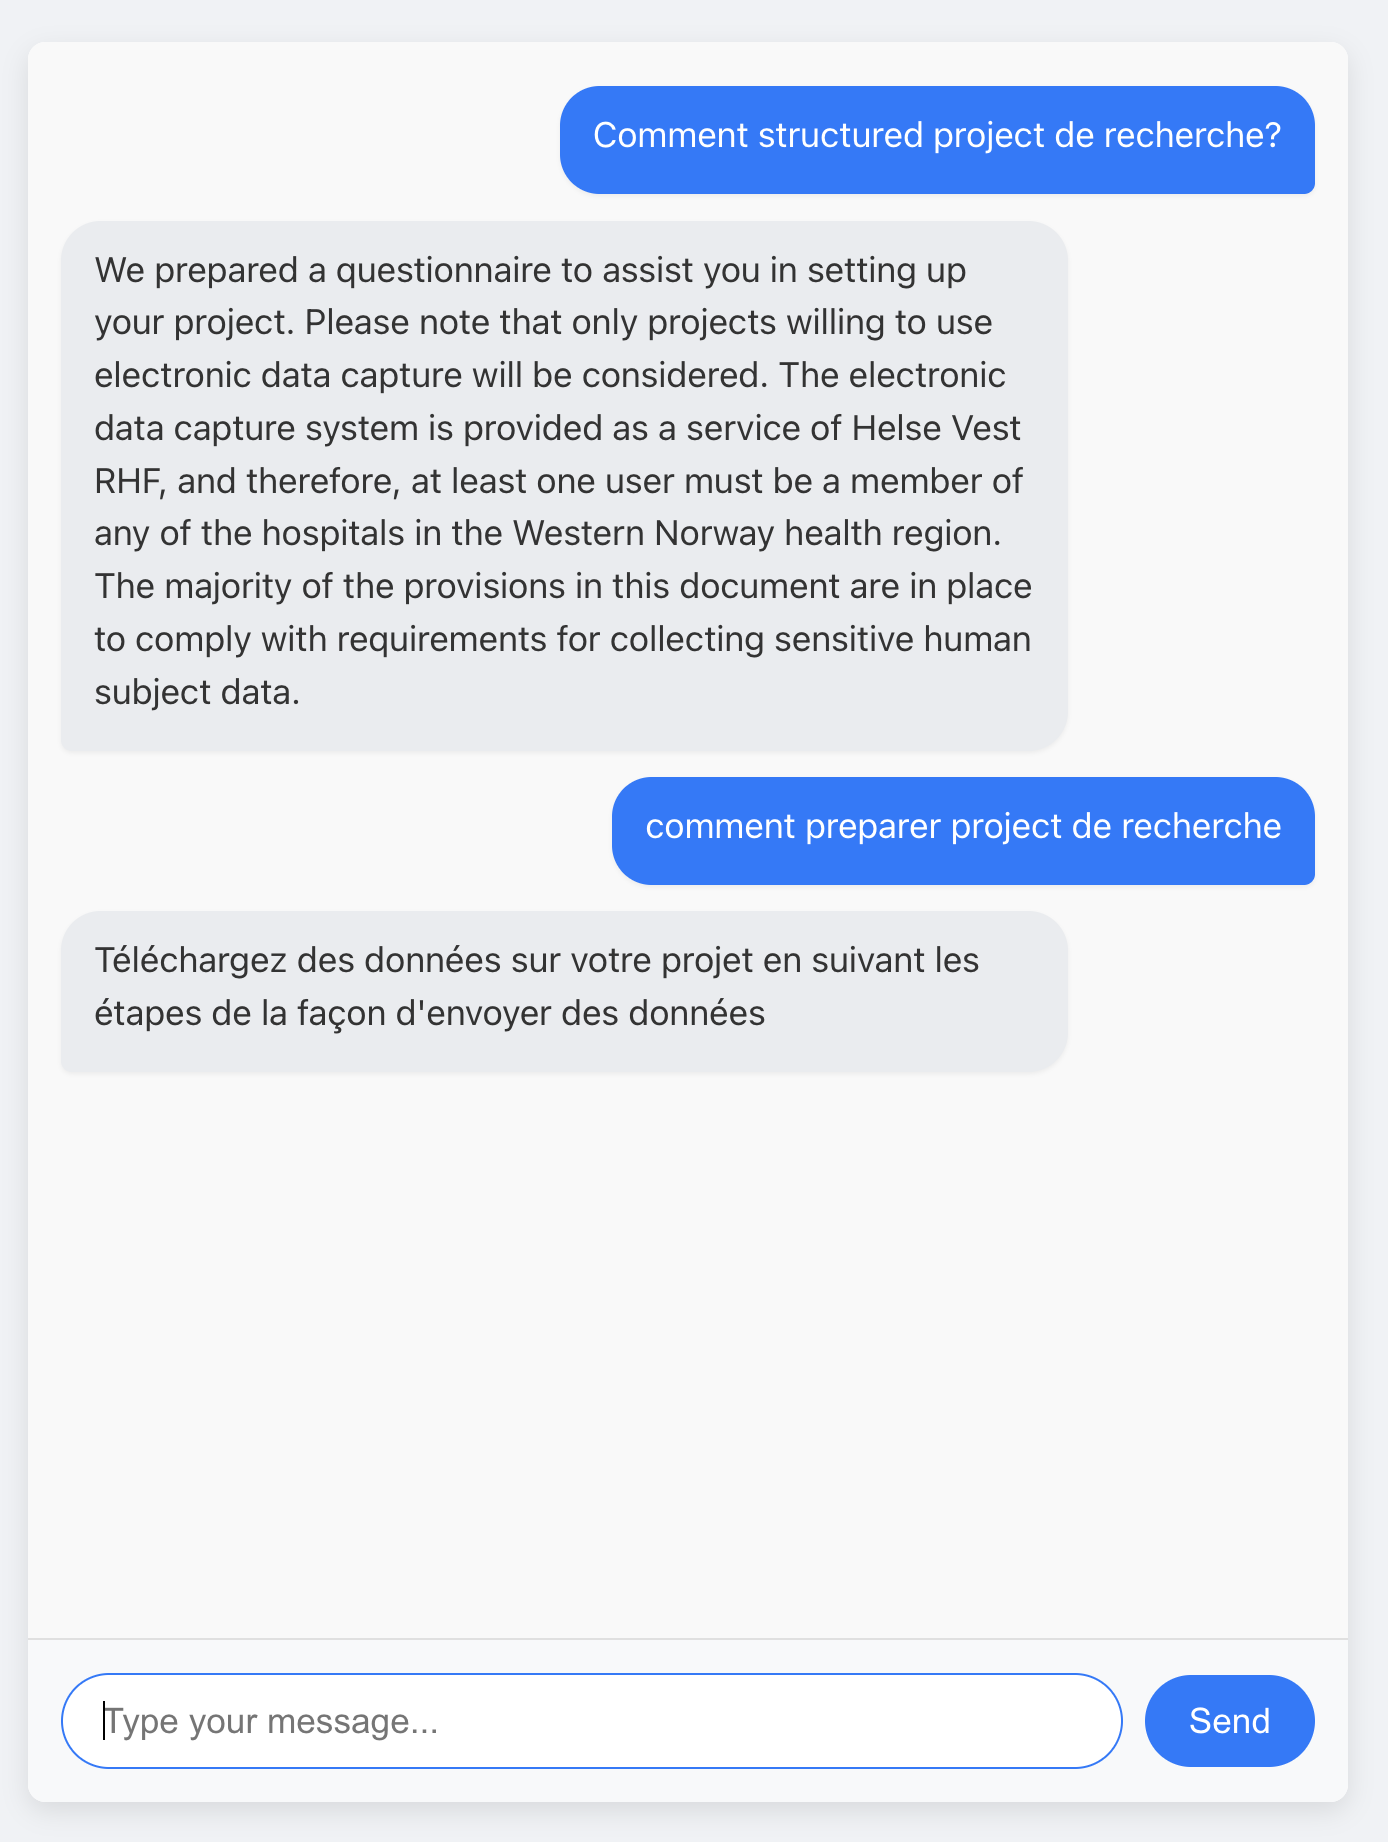
\includegraphics[width=\textwidth]{ui-screenshot.png}
    \note{
        The frontend uses `Chat.js` for the main interface and communicates with the backend via HTTP POST requests. Styling is managed with `Chat.css` and `styles.css`.
    }
\end{frame}

\begin{frame}{Integration with Apache2 and PHP 8.x}
    \begin{itemize}
        \item Backend can be proxied through Apache2 for seamless integration.
        \item Frontend served as static files (build directly) with PHP existing code.
        \item Supports integration with PHP 8.4.6.
        \item Run chatbot integrated with existing PHP code: http://localhost:8080/index.php
    \end{itemize}
    \note{
        Apache2 acts as a reverse proxy for the backend, while the frontend is served as static files. This setup ensures compatibility with PHP-based enterprise systems.
    }
\end{frame}

\end{document}
